%%%%%%%%%%%%%%%%%%%%%%%%%%%%%%%%%%%%%%%%%%%%%%%%%%%%%%%%%
%                                                       %
%           Validation Sheet of Code_Saturne            %
%                      CYCLONE                          %
%                                                       %
%%%%%%%%%%%%%%%%%%%%%%%%%%%%%%%%%%%%%%%%%%%%%%%%%%%%%%%%%

% -------------------------------
% DEFINITION OF PRACTICAL LENGTHS
% -------------------------------
\newlength{\largfigpp}
\setlength{\largfigpp}{4.5cm}
\newlength{\largfigk}
\setlength{\largfigk}{6.5cm}
\newlength{\largfigp}
\setlength{\largfigp}{8cm}
\newlength{\largfign}
\setlength{\largfign}{10cm}
\newlength{\largfigm}
\setlength{\largfigm}{12cm}
\newlength{\largfigt}
\setlength{\largfigt}{13cm}
\newlength{\largfigi}
\setlength{\largfigi}{14cm}
\newlength{\largfigg}
\setlength{\largfigg}{16cm}
\newlength{\largleg}
\setlength{\largleg}{12cm}

\renewcommand{\IMAGES}{./IMAGES}

\chapter{STAIRMAND Cyclone}

\sousti{Alexandre Douce (2001), RENUDA}{8/10/2020}
\keywords{Incompressible, Lagrangian Two-Phase, Turbulent ($R_{ij}-\varepsilon~SSG$), one-way and two-way coupling.}

\section{Test Case Description}

\subsection{Purpose}

In general, the cyclones are an example of a two-phase separator which are used to separate solid particles contained in a gas flow into two flows: the gas which
leaves the cyclone through the upper exit and the particles which are collected at the bottom of the cyclone.

\noindent
Within this validation test case, the air turbulent flow in the cyclone is simulated without and with an injection of particles. The correct prediction of the monophasic simulation is essential for the evaluation of the separating power of the device (aspect which generally constitutes the ultimate goal of studies).

The goal of this study is to check if the turbulence model $R_{ij}-\varepsilon~SSG$ established in \CS predicts the "double spin" structure of the flow.


\subsection{Setup Description}


The geometry is presented in figure \ref{schema}.

\begin{figure}[H]
   \centerline{\includegraphics[width=15cm]{\IMAGES/cycl.eps}}
   \caption{Test case geometry.}
   \label{schema}
\end{figure}

The fluid inlet is tangential to the axis of the cylinder. The flow then goes down along the
spiral wall to the bottom of the cyclone, then the fluid goes up through the central part of the cyclone in order to
exit through the upper outlet. The geometrical characteristics of the Stairmand cyclone are summarized
in table \ref{fig2_cycl}:


\begin{table}[!h]
\begin{center}
\begin{tabular}{|c|c|c|c|c|c|c|c|}
\hline
D $(mm)$ & De $(mm)$ & H $(mm)$ & h $(mm)$ & a $(mm)$ & b $(mm)$ & S $(mm)$ & B $(mm)$ \\
\hline
200 & 100 & 800 & 300 & 100 & 40 & 100 & 72 \\
\hline
\end{tabular}
\end{center}
\caption{Dimensions of the Stairmand cyclone. }
\label{fig2_cycl}
\end{table}

The particles are injected all at the same time \cite{Peirano}. 

\subsection{Fluid caracteristics}

\begin{itemize}
\item[$\bullet$] Cinematic viscosity : $\nu~=~10^{-5}~m^2\cdot s^{-1}$
\item[$\bullet$] Density : $\rho~=~1~kg/m^3$
\item[$\bullet$] Volumic flow rate of $0.12~m^3/s$ is imposed at the inlet corresponding to a reference velocity of $U_0~=~30~m\cdot s^{-1}$ (inlet velocity). 
\item[$\bullet$] Reynolds number : $Re~=~U_0\cdot De/\nu~=~3\cdot10^5$
\end{itemize}

Remarks : A volumic flow rate imposed at the inlet gives better results than a uniform velocity.

\subsection{Particles caracteristics}

The particles have a density of $2500~kg/m^3$ and their diameters are ranging between $0.5$ and $5~mm$.

\subsection{References}

\begin{thebibliography}{3}

\bibitem{ficheestet} Matt\'ei J.-D., Picard N.,\\
``Syst\`eme ESTET-ASTRID Tome I : Application au monophasique.\\
Recueil de fiches de validation ESTET - Version 3.4'',\\
{\it Rapport EDF}, HI-83/00/008, 2000.

\bibitem{Boysan83} F. Boysan, B.C.R. Ewan, J. Swithenbank and W.H. Ayers\\
``Experimental and theoretical studies of cyclone separators aerodynamics'',\\
{\it I. Chem. E., POWTECH Conference}, 1983.

\bibitem{Davroux00} A. Davroux, F. Archambeau\\
``Le $R_{ij}-\varepsilon$ dans \CS \ (version $\beta$)'',\\
{\it Rapport EDF}, HI-83/00/030, 2000.

\bibitem{Peirano} E. Peirano, S. Chibbaro, J. Pozorski, J.-P. Minier \\
``Mean-field/PDF numerical approach for polydispersed turbulent two-phase flows'',\\
{\it Progress in Energy and Combustion Science}, 315–371, 32 (2006).

\end{thebibliography}

% =============================
\section{Numerical setup}
% =============================

\subsection{Numerical modelling}

\begin{itemize}

   \item \textbf{Type of calculation} :
         \begin{itemize}
            \item[$\rightarrow$] Continuous phase: incompressible, turbulent, 3D, High Reynolds.
            \item[$\rightarrow$] Dispersed phase: solid particles, one-way coupling.
            \item[$\rightarrow$] Dispersed phase: solid particles, two-way coupling.
         \end{itemize}

   \item \textbf{Gravity}: No

   \item \textbf{Turbulence model}: $R_{ij}-\varepsilon~SSG$
   
   \item \textbf{Passive scalar}: a passive scalar is introduced at the inlet to follow the "convergence" of the
calculation; as it does not represent any physical quantity, it is not referred to in the rest of
the study.


\end{itemize}

\subsection{Mesh}

\begin{description}

\begin{figure}[H]
   \centerline{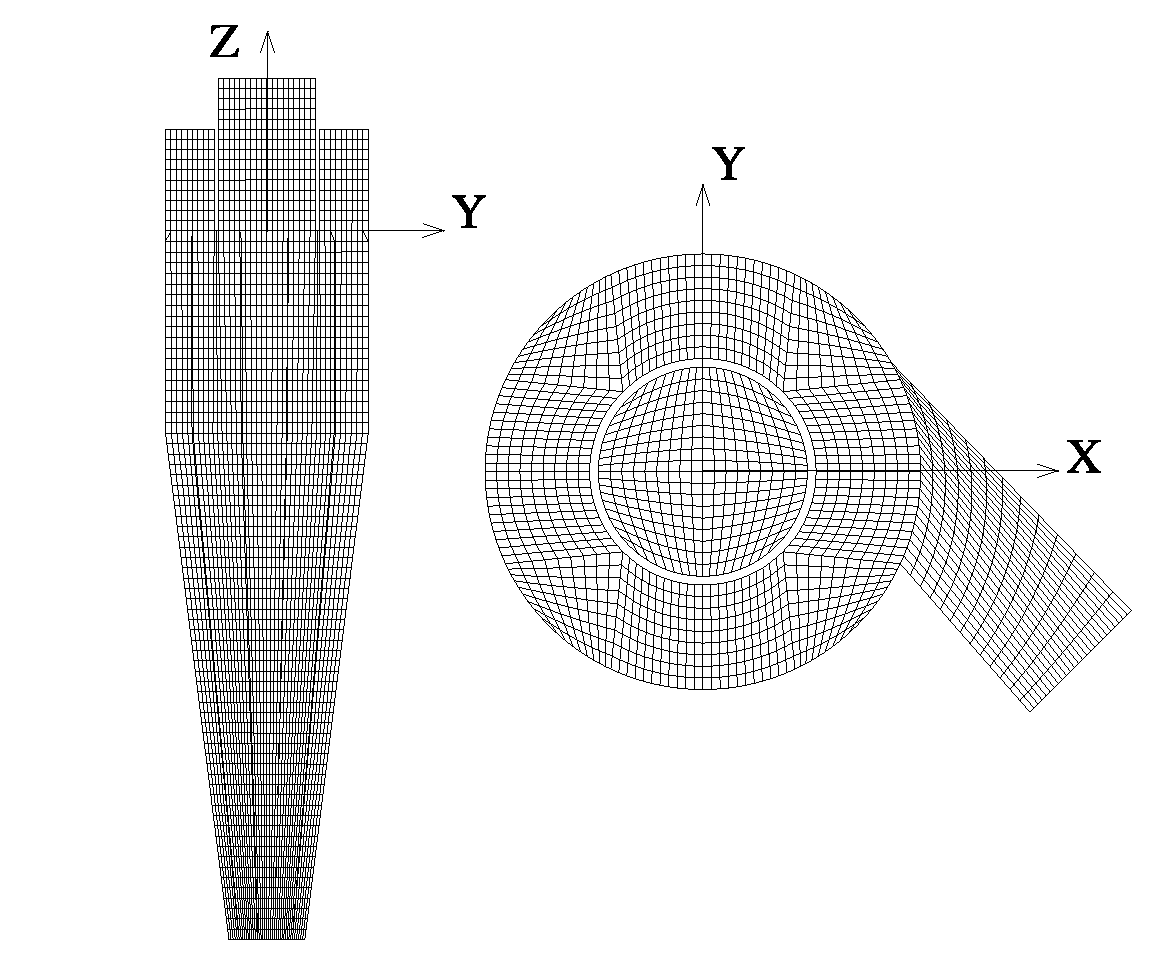
\includegraphics[width=15cm]{\IMAGES/maillage2D.eps}}
   \caption{Clips of the mesh.}
   \label{mail2D}
\end{figure}

\begin{figure}[H]
   \centerline{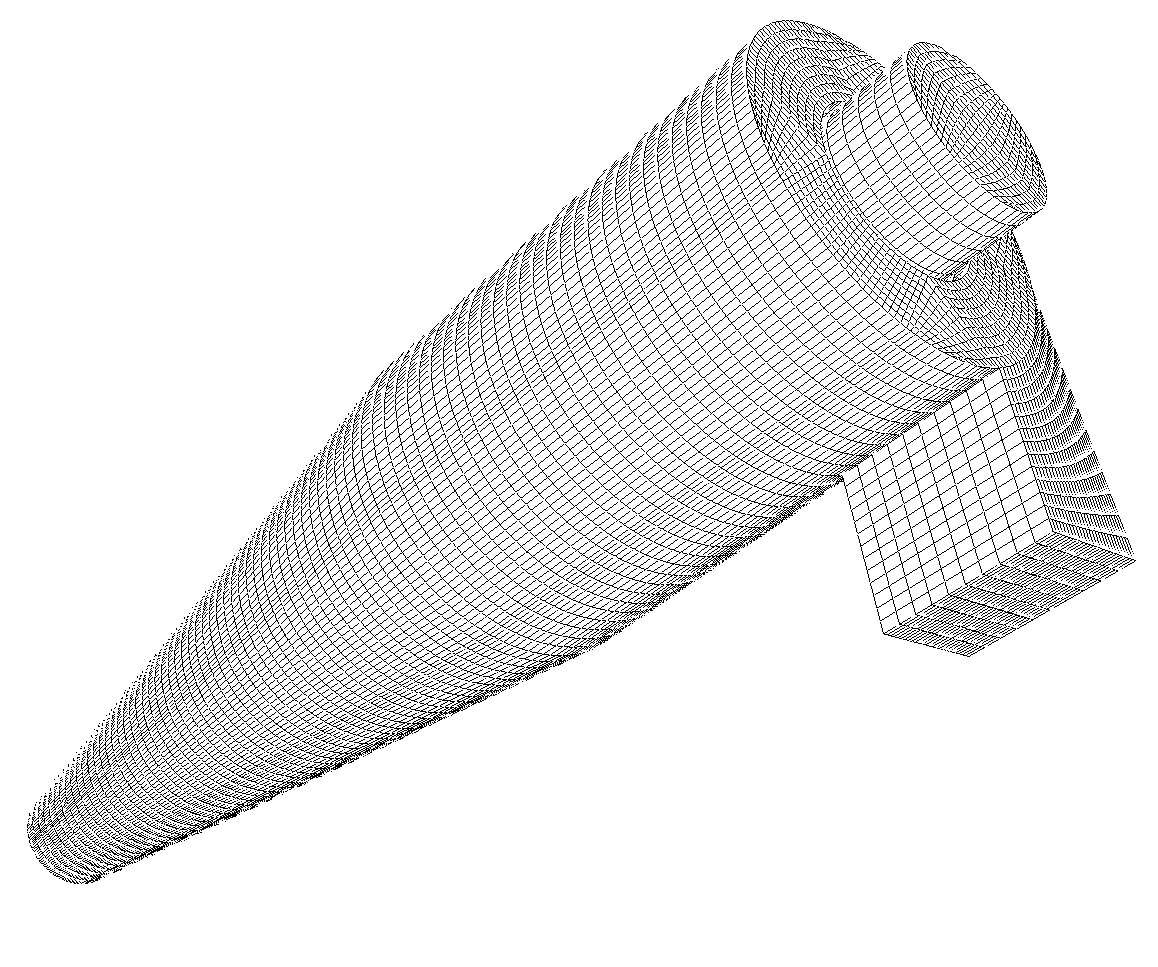
\includegraphics[width=15cm]{\IMAGES/maillage3D.eps}}
   \caption{Mesh.}
   \label{mail3D}
\end{figure}

   \item[\textbf{Coordinate system}:] Cartesian, origin at the bottom of the output skirt, and in the center of the cylinder (see fig \ref{mail2D})

   \item[\textbf{Process used to build the mesh} :] it is a mesh generated with ESTET, which has been transformed via the ESTET2SOLCOM tool into a geometric data file directly
usable by \CS.




\end{description}

\noindent{\textbf{Number of cells} :} 128,070 \\
\noindent{\textbf{Number of internal faces} :} 376,936 \\
\noindent{\textbf{Number of boundary faces} :} 18,550 \\

\noindent 
The beginning of the listing of \CS gives the angles of non-orthogonality of the mesh:
\scriptsize
\begin{verbatim}
 HISTOGRAMMES DES ANGLES DE NON ORTHOGONALITE

   Faces internes
      00-15     15-30     30-45     45-60     60-75     75-90
     232013    112316     23006      7021      2580         0

   Faces de bord
      00-15     15-30     30-45     45-60     60-75     75-90
       9688      3251      2061      1398      1408       744
\end{verbatim}
\normalsize
We note that a certain number of elements have high non-orthogonality angles, which means that it is a medium quality mesh. This is due to the presence of strongly "flattened" cells
on the wall (figure \ref{mail3D}).

\subsection{Boundary and Initial Conditions}

\begin{itemize}

\item[$\bullet$] \textbf{Fluid boundary conditions} :

\begin{table}[H]
   \begin{center}
      \begin{tabular}{lccc}
         \hline\hline
            BC & Name & Fluid boundary conditions  \\      
         \hline
         BC\_1 & Inlet 	& inlet \\
         BC\_2 & Outlet\_up 	& outlet \\
         BC\_3 & Walls		& wall \\
         BC\_4 & Outlet\_bot 	& outlet \\
         \hline\hline
      \end{tabular}
   \end{center}
\end{table}


\item[$\bullet$] {\textbf{ Conditions for the velocity} $\textbf{u}=(u,v,w)$}
\begin{description}
\item[]{\textbf{ Inlet} :} Dirichlet condition :
\begin{description}
\item[-] volumic flow rate of $0.12~m^3/s$ is imposed at the inlet corresponding to a reference velocity of $U_0~=~30~m\cdot s^{-1}$
\end{description}
\item[]{\textbf{ Outlets} :} standard free outlet type 9.
\item[]{\textbf{ Walls} :} friction condition (wall model with two 2 scale model).
\item[]{\textbf{ Initial Conditions} :} $u=0~;~v=0~;~w=0$.
\end{description}

\item[$\bullet$] {\textbf{ Boundary conditions for the pressure}}
\begin{description}
\item[]{\textbf{ Free Outlets} :} Dirichlet (standard, {\em i.e.} as
$\frac{\partial}{\partial n}\frac{\partial P}{\partial \tau}=0$).
\item[]{\textbf{ Elsewhere} :} homogeneous Neumann.
\end{description}

\item[$\bullet$] {\textbf{ Conditions for the scalars}}
\begin{description}

\item[-]{\it Variables for the turbulence}
%
\newline
The values for the turbulence are calculated from the hydraulic diameter for the inlet and all the other default parameters are calculated by \CS.

\begin{description}
\item[]$S$, Inlet section, is $4\cdot10^{-3}~m^2$,
\item[]$P$, Wet perimeter, is $0.28~m$,
\item[]$D_h$, Hydraulic diameter, is : $\frac{4\cdot S}{P} = 0.057~m$,
\item[]$Re_H$, Reynolds number based on the hydraulic diameter, is : $Re_H=\frac{U\cdot D_H}{\nu}$, so $Re_H=1.7\cdot10^5$
\item[]$\lambda$ is so $0.184 Re_H^{-0.2}$, so $\lambda =0.016$
\item[]and we obtain $u*=\sqrt{\frac{\lambda}{8}}U$ with $U=30~m \cdot s^{-1}$, so $u*~=~1.36~m\cdot s^{-1}$.
\end{description}

\item[]{\textbf{ Inlet} :} Dirichlet condition
\item[]{\textbf{ Outlets} :} Standard free outlet
\item[]{\textbf{ Walls} :} Condition for a turbulent wall. 
\item[]{\textbf{ Initial conditions} :} calculated from $U_{ref}=U_{0}$.
\end{description}

\item[-]{\it Passive scalar}

\begin{description}
\item[]{\textbf{ Inlet} :} Dirichlet condition (value = 1) 
\item[]{\textbf{ Elsewhere} :} homogeneous Neumann. 
\item[]{\textbf{ Initial conditions} :} null value.
\end{description}

\item[$\bullet$] \textbf{Particle boundary conditions} :
%
\begin{table}[H]
   \begin{center}
      \begin{tabular}{lccc}
         \hline\hline
            BC & Name & Particle boundary conditions           \\      
         \hline
         BC\_1 & Inlet 	& inlet \\
         BC\_2 & Outlet\_up 	& outlet \\
         BC\_3 & Walls		& perfect rebound \\
         BC\_4 & Outlet\_bot 	& outlet \\
         \hline\hline
      \end{tabular}
   \end{center}
\end{table}

The diameter range of the particles has been discretised as follows, [$0.5$; $1$; $1.5$; $2$; $3$; $4$; $5$]$~mm$.
For each class (diameter of particles), a number of $100$ particles is released (this number is identical for each
class).

\end{itemize}

\subsection{Numerical schemes}

For the two turbulence models, all the numerical parameters are those defined by default
in \CS. We use a centered-upwind scheme, configured to be $100\%$ centered (\texttt{BLENCV=1}), as the convection scheme.

\subsection{User coding}

\begin{description}

   \item[-] \textbf{cs\_user\_extra\_operations.f90} : in order to change the time step for a one-phase calculation (from $10^{-4}$ to $10^{-5}~s$) in order to avoid a jump during the restart for the two-phase calculation.

\end{description}

\subsection{Calculation strategy}

The runs are carried out in two steps. The first step is a one-phase calculation, without particles. This makes it possible to initialise the two-phase calculations. During the one-phase calculation, the time step is reduced in order to avoid a jump at the restart for the two-phase calculations. Because the particles are injected at the beginning of the two-phase calculations, it was important to avoid the jump at the restart. \\ 

\begin{description}

   \item[$\bullet$]\textbf{One-phase calculation}
         \begin{itemize}
            \item[-] {\bf Restart:} NO
            \item[-] {\bf Maximum time :} $0.8~s$
            \item[-] {\bf Time step: constant (\texttt{IDTVAR=0}), } $10^{-4}~s.$ then $10^{-5}~s.$ after $t~=~0.5~s$
         \end{itemize}


   \item[$\bullet$]\textbf{Two-phase calculation - One Way}
         \begin{itemize}
            \item[-] {\bf Restart:} YES
            \item[-] {\bf Restart of the Lagrangian calculation:} NO
            \item[-] {\bf Total number of time steps (including one-phase calculation):} 100,000
            \item[-] {\bf Time step: (\texttt{IDTVAR=0}),} $10^{-5}~s$
            \item[-] \textbf{Stationary continuous phase:} NO (\texttt{ISTTIO=0})

            \item[-] {\bf Turbulent dispersion model:}
                  \begin{itemize}
                     \item[*] For the two-phase calculation, the default complete model with the local rotation option is utilised.

                  \end{itemize}
            \item[-] {\bf Dynamic one-way coupling:} YES (\texttt{IILAGR=1} and \texttt{LTSDYN=1})

            \item[-] {\bf Total number of class for particles:} 7
            \item[-] {\bf Total number of particles injected for each class and at the first lagrangian iteration:} 100
         \end{itemize}

   \item[$\bullet$]\textbf{Two-phase calculation - Two Way}
         \begin{itemize}
            \item[-] {\bf Restart:} YES
            \item[-] {\bf Restart of the Lagrangian calculation:} NO
            \item[-] {\bf Total number of time steps (including one-phase calculation):} 100,000
            \item[-] {\bf Time step: (\texttt{IDTVAR=0}),} $10^{-5}~s$
            \item[-] \textbf{Stationary continuous phase:} YES (\texttt{ISTTIO=1})

            \item[-] {\bf Turbulent dispersion model:}
                  \begin{itemize}
                     \item[*] For the two-phase calculation, the default complete model with the local rotation option is utilised.

                  \end{itemize}
            \item[-] {\bf Dynamic two-way coupling:} YES (\texttt{IILAGR=2} and \texttt{LTSDYN=1})

            \item[-] {\bf Total number of class for particles:} 7
            \item[-] {\bf Total number of particles injected for each class and at the first lagrangian iteration:} 100
         \end{itemize}

\end{description}

% =============================
\section{Results}
% =============================

\subsection{Run data}

\begin{description}

   \item[$\bullet$]\textbf{One-phase run}

         \begin{itemize}
            \item[$\bullet$] Inlet flow at the outlets: NO
            \item[$\bullet$] Number of clips on $R_{ij}-\varepsilon$ in the listing: none
            \item[$\bullet$] Maximum CFL number of the order of 0.4 (very stable)
         \end{itemize}

   \item[$\bullet$]\textbf{Two-phase run - One way coupling}

         \begin{itemize}
            \item[$\bullet$] Inlet flow at the outlets: NO
            \item[$\bullet$] Number of clips on $R_{ij}-\varepsilon$ in the listing: none
            \item[$\bullet$] Maximum CFL number of the order of 0.4 (very stable)
            \item[$\bullet$] Percentage of lost particles: $0.0$\%
         \end{itemize}
         
   \item[$\bullet$]\textbf{Two-phase run - Two way coupling}

         \begin{itemize}
            \item[$\bullet$] Inlet flow at the outlets: NO
            \item[$\bullet$] Number of clips on $R_{ij}-\varepsilon$ in the listing: none
            \item[$\bullet$] Maximum CFL number of the order of 0.4 (very stable)
            \item[$\bullet$] Percentage of lost particles: $0.0$\%
         \end{itemize}

\end{description}

\subsubsection{Convergence}

\begin{description}

   \item[$\bullet$]\textbf{One-phase run convergence}

Figure \ref{transit_cycl} gives the evolution of the axial component of velocity at five points, $C_i$ (see the probe locations in the figure \ref{local_cycl} and the table \ref{tab1_cycl} to see the corresponding probe numbers).

\parbox{0.55\textwidth}{
\begin{figure}[H]
\centerline{\includegraphics[width=5cm]{\IMAGES/poscapt.eps}}
\caption{\textit{Probe locations.}\label{local_cycl}}
\end{figure}}
\parbox{0.35\textwidth}{
\begin{table}[H]
\begin{center}
\begin{tabular}{|c|c|ccc|}
\hline
$Probe$ & $Probe~number$ & $X$ & $Y$ & $Z$ \\
\hline
$C_1$&$1$&0&0&-0.20\\
\hline
$C_2$&$2$&0&0&0\\
\hline
$C_3$&$3$&0&0.05&-0.1\\
\hline
$C_4$&$4$&0.05&0&-0.1\\
\hline
$C_5$&$5$&0.07&-0.07&0.05\\
\hline
\end{tabular}
\caption{Coordinates of the probes (in $m$)\label{tab1_cycl}}
\end{center}
\end{table}}

The figures below show the evolution of the convergence rate for $0.8~s$. We note the jump at $t~=~0.5~s$ when the time step is reduced from $10^{-4}~s$ to $10^{-5}~s$. The simulation exhibits oscillations around the mean values. 

\begin{figure}[H]
\centerline{\includegraphics[width=7.0cm]{\IMAGES/VNV/probes_MONO_RIJ.pdf}}
\caption{One-phase calculation - Evolution of the axial velocity}
\label{transit_cycl}
\end{figure}

   \item[$\bullet$]\textbf{Two-phase run convergence - One way coupling}

The figures below shows the evolution of the convergence rate for the one way coupling calculation. The simulation exhibits oscillations around the mean values. 

\begin{figure}[H]
\centerline{\includegraphics[width=7.0cm]{\IMAGES/VNV/probes_DIPH_RIJ_OneWay.pdf}}
\caption{Two-phase calculation - One way coupling - Evolution of the axial velocity}
\label{transit_cycl_one_way}
\end{figure}

   \item[$\bullet$]\textbf{Two-phase run convergence - Two way coupling}

The figures below show the evolution of the convergence rate for the two way coupling calculation. The simulation exhibits oscillations around the mean values. 

\begin{figure}[H]
\centerline{\includegraphics[width=7.0cm]{\IMAGES/VNV/probes_DIPH_RIJ_TwoWay.pdf}}
\caption{Two-phase calculation - Two way coupling - Evolution of the axial velocity}
\label{transit_cycl_two_way}
\end{figure}

\end{description}

\subsection{Results}

Due to the fluctuations in the flowfield (seen in \ref{transit_cycl}, \ref{transit_cycl_one_way}, and \ref{transit_cycl_two_way}), the velocity fields are time averaged from $t~=~0.6~s$ to $0.8~s$ for the one-phase calculation and from $t~=~0.9~s$ to $1.45~s$ for the two-phase calculations. Figures \ref{vit_ax} and \ref{vit_tg} present the profiles of the axial and tangential components of the instantaneous velocity in the cyclone according to horizontal sections for which experimental measurements are available in \cite{Boysan83} at the last time step of the calculations, and the figures \ref{Time_avg_vit_ax} and \ref{Time_avg_vit_tg} present the same profiles with a time average.

\begin{figure}[H]
\centerline{\includegraphics[width=15cm]{\IMAGES/VNV/Axial_velocity.pdf}}
\caption{Axial velocity of the single and two-phase calculations compared to the experiment}
\label{vit_ax}
\end{figure}

\begin{figure}[H]
\centerline{\includegraphics[width=15cm]{\IMAGES/VNV/Tangential_velocity.pdf}}
\caption{Tangential velocity of the single and two-phase calculations compared to the experiment}
\label{vit_tg}
\end{figure}

\begin{figure}[H]
\centerline{\includegraphics[width=15cm]{\IMAGES/VNV/Time_avg_Axial_velocity.pdf}}
\caption{Time averaged axial velocity of the single and two-phase calculations compared to the experiment}
\label{Time_avg_vit_ax}
\end{figure}

\begin{figure}[H]
\centerline{\includegraphics[width=15cm]{\IMAGES/VNV/Time_avg_Tangential_velocity.pdf}}
\caption{Time averaged tangential velocity of the single and two-phase calculations compared to the experiment}
\label{Time_avg_vit_tg}
\end{figure}

Figure \ref{num_part} presents the number of particles during the two-phase calculations. Figure \ref{part_bot} presents the proportion of the total particles injected in the domain going through the bottom outlet depending on the class of particles (the diameter range of the particles is [$0.5$; $1$; $1.5$; $2$; $3$; $4$; $5$]$~mm$).

\begin{figure}[H]
\centerline{\includegraphics[width=15cm]{\IMAGES/VNV/Number_of_particles.pdf}}
\caption{Number of particles}
\label{num_part}
\end{figure}

\begin{figure}[H]
\centerline{\includegraphics[width=10cm]{\IMAGES/VNV/Outlet_bottom.pdf}}
\caption{Particles going through the bottom outlet}
\label{part_bot}
\end{figure}

 
\subsection {Analysis and discussion}

The flow field has an unsteady character in the simulations as seen experimentally in \cite{Boysan83}. This is the reason why the computed flow fields were time averaged in order to plot the axial and tangential velocity components. The one-phase and the two-phase calculations produce, as expected, similar profiles for the axial and tangential velocity at different horizontal sections. The axial velocity component has a negative value at the center of the cyclone which is higher than the experimental one. For the two-way coupling calculation, the particles do not have a visible impact on the flow field. The axial velocities are accurately predicted at $z~=~0.6$ and $0.57~m$ whereas the tangential velocities show a shift of the radius where there is the maximum tangential velocity between the experiment and the simulations. Based on the experimental data, the maximum tangential velocities are located at around $r~=~0.02$ and $r~=~0.05m$, depending on the $z$ coordinate, while the simulations predict the locations of the maximum tangential velocities at around $r~=~0.01$ and $r~=~0.02m$. Between the maximum tangential velocities and the walls, the slopes of the velocity profiles are similar to those of the experiment.

For the two-phase calculations, the evolution of the number of particles is similar between the one-way and the two-way coupling solutions. The proportion of the total particles injected in the domain going through the bottom outlet, depending on the class of particles, has a similar selectivity curve in the one-way and the two-way coupling (i.e. around class 5 corresponding to a diameter of particles of $3~mm$). Only for the secong class ($1~mm$) the two-way coupling has more particles going through the bottom outlet than the one-way calculation, but it is important to note that this difference of the selective curve around the second or the third class changes from one run to another.

In order to better understand the structure of the flow, a visual examination of several physical moments
was done in a vertical section plane. We have thus been able to observe that model $R_{ij}-\varepsilon~SSG$ manages to reproduce the characteristic vertical velocity reversal at the bottom of the cyclone
(unsteady). In addition, it can be seen that the double spin is not stabilized on the axis of the
cyclone, but on the contrary moves in the vicinity of this axis.

In conclusion, the results obtained for this industrial case have the expected characteristics. In addition, it would be interesting to do a mesh dependency and time step analysis computations to see the impact on the selectivity curve.


\clearpage

\section{Archiving}

The directory for the case is named: \textbf{CYCLONE}

The sub-directories are organised as follows:
\medskip\\
\hspace*{2cm}\textbf{RIJ}: everything having to do with the single-phase calculation.
\medskip\\
\hspace*{2cm}\textbf{DIPH\_OneWay}: everything having to do with the two-phase calculation in one way coupling.
\medskip\\
\hspace*{2cm}\textbf{DIPH\_TwoWay}: everything having to do with the two-phase calculation in two way coupling.

